% !TeX root = ../relazione.tex

\chapter{SQLite Recovery}
SQLite Recovery è uno script scritto in python nella versione 3.8.10.  

Quest'ultimo permette di recuperare i record cancellati, più nello specifico utilizza lo spazio non allocato delle pagine foglie b-tree di tipo tabelle e dei freeblock presenti nelle pagine di questo tipo.

Lo script è stato testato su file SQLite del formato 3.

Lo strumento opera in due modalità che saranno eseguite entrambe ad ogni esecuzione.

La prima modalità si limiterà a prendere i dati delle aree in cui potrebbero essere presenti dei record e li immagazzinerà in un file chiamato raw\string_data.tsv.

La seconda modalità, a partire dai dati ottenuti dalla modalità precedente, cercherà di parsare i record o frammenti di record.

Terminata l’esecuzione sarà possibile visualizzare i record ottenuti tramite il file “report.html” (assicurarsi che il browser utilizzato per l’apertura del file html permetta il caricamento di file json locali), per maggiori informazioni visitare la pagina GitHub \footnote{GitHub repository: \url{https://github.com/Er-Simon/Sqlite3-restore-deleted-records}}.


\section{Ambiente di testing}
Per testare il corretto funzionamento dello script, è stato realizzato attraverso l'ausilio dell'applicazione di messaggistica istantanea Whatsapp un ambiente di testing. Innanzitutto, è stato creato un account attraverso il quale è stata simulata una conversazione con un altro account. Durante questa conversazione c'è stato uno scambio di un totale di 11 messaggi, dei quali 4 di tipo testo, 3 immagini di cui una con la descrizione, 2 messaggi vocali e 2 contatti.

Successivamente sono stati rimossi diversi messaggi: una delle 3 immagini scambiate, un contatto e un messaggio vocale.

Prima della rimozione è stato esportato il file SQLite generato dall'applicazione di Whatsapp ed è stato eseguito il comando vacuum per vedere se ricostruendo il database fosse cambiata la dimensione, in modo da capire se ci fossero già eventuali tracce (come i freeblock, i dati nelle aree non allocate o delle pagine inattive). Eseguito il comando, la dimensione è rimasta invariata.

È stato eseguito nuovamente il comando dopo l'eliminazione e si è notato che il file ottenuto era di diversa dimensione. Raggiunto questo risultato si è compreso che qualche messaggio eliminato dovesse essere ancora presente all'interno del file, ma contrassegnato come rimosso.

\section{Patterns}
Precedentemente è stata illustrata la procedura di recupero dei record. Come si è notato, il recupero ha permesso di ottenere le informazioni su i tipi di dati contenuti nelle celle e il contenuto di quest'ultime.
Sulla base delle informazioni ottenute dall'intestazione del record (ovvero i tipi dei campi) e presupponendo che queste informazioni siano corrette, verrà illustrato il procedimento per costruire per ogni record un insieme di tabelle candidate di appartenenza. 
Prima di tutto lo script analizzerà lo schema del database per ricavare per ogni tabella un pattern sul tipo di dati delle celle. Per ogni tabella verrà quindi preso il nome, il numero di campi da cui è costituita e per ogni campo verrà preso il nome e i suoi flag, cioè se primary key, se not null e il tipo di dato.
Ottenute queste informazioni, si è in grado di costruire un insieme di tabelle candidate per ogni record trovato, basandosi sul confronto cella per cella con le informazioni ottenute dallo schema.
Una ricerca di questo tipo potrebbe produrre anche falsi risultati: si potrebbe pensare di includere come criterio di ricerca anche l'id del record e confrontarlo con gli id delle righe non eliminate presenti all'interno del database.

\section{Risultati ottenuti}
Eseguito lo script adottando il criterio di ricerca precedentemente illustrato si è arrivati a un numero cospicuo di record e di tabelle candidate, bisogna però considerare che il database di Whatsapp è costituito da 36 tabelle molte delle quali con lo stesso schema.

Molti dei record trovati sono falsi positivi, in quanto, l'intestazione del record eliminato non risultava essere intatta. Tra i record trovati però ci sono anche i record relativi ai messaggi eliminati.
Più nello specifico si sono recuperati i record rappresentanti l'invio del contatto Whatsapp, in cui sono presenti le informazioni relative a quando è avvenuto il messaggio, il mittente, il destinatario e le informazioni sul contatto (nome, numero di cellulare, ecc..).
Whatsapp solo per questo messaggio ha generato 4 record in 4 differenti tabelle.
Il record rimosso contente queste informazioni è stato recuperato all'interno dell'area non allocata di una pagina.
Inoltre, sono stati recuperati anche i record generati a seguito dell'invio dell'immagine e le relative informazioni, come il path in cui è situtata all'interno del dispositivo, quando è stato inviato il messaggio, il mittente e il destinatario, la thumbnail dell'immagine, la grandezza in byte e molte altre informazioni.
I record relativi all'immagine sono stati trovati sia nelle aree non allocate che nei freeblock.
Mentre, per quanto riguarda il messaggio vocale, lo script non è stato in grado di recuperare alcun record.

Per avere un ulteriore riscontro sul corretto recupero dei record, dono stati confrontati i risultati ottenuti con un altro software chiamato FQLite \cite{fqlite}.
Visionando i risultati ottenuti da entrambi i software, si è notato che FQLite, a differenza dello script SQLite Recovery, ha trovato meno record falsi positivi, ma, per quanto riguarda i record validi, sono stati trovati gli stessi record da entrambi.
Questo dovrebbe essere dovuto al fatto che FQLite nel criterio di ricerca include anche il confronto della chiave primaria della riga trovata, con le chiavi primarie delle righe presenti nelle tabelle candidate.

\section{Implementazione}
I file riportati di seguito fanno riferimento alla repository GitHub menzionata in precedenza.

\medskip

Il file main.py utilizzerà la variabile database\string_path per contenere il path in cui è collocato il file del database.

\medskip

Verrà creato un oggetto della classe database (database\string_parser.py) rappresentante il file situato al database\string_path, durante la creazione verificherà che il file esista, otterrà la dimensione in byte del file e verrà controllato che l’utente abbia i permessi di lettura. 
Se le condizioni precedenti sono verificate procederà ad aprire il file in modalità “rb” (reading binary) e ne leggera i primi 100 byte (l’header del database).
Tramite l’header controllerà che i primi 16 byte convertiti in hex corrispondano alla stringa “53514c69746520666f726d6174203300”, in quanto ogni SQLite database file valido inizia con i precedenti byte.
Leggerà i successivi 2 byte (offset 16) per acquisire la grandezza delle pagine in byte e successivamente all’offset 56 ne leggerà ulteriori 4 per ottenere un intero rappresentante la codifica utilizzata per immagazzinare le stringhe nel database.

\medskip

Terminata la fase di inizializzazione verrà creato un oggetto della classe report presente nel file (report\string_builder.py). Questo oggetto rappresenta le informazioni ottenute durante l’esecuzione dello script, inoltre, al termine dell’esecuzione genererà un file “report.html” per visualizzare le informazioni ottenute.

\medskip

Aperto il flusso di dati del file e ottenute le informazioni essenziali per operare avrà luogo la prima modalita;

\medskip

Verrà aperto in scrittura il file raw\string_data.tsv in cui saranno scritte le informazioni raccolte.
Verrà letto il file specificato da database\string_path fino alla fine andando ad incrementare l’offset ad ogni lettura di un numero di byte pari alla grandezza di una pagina, così facendo ogni volta andremo a lavorare su una diversa pagina alla volta.

\medskip

Per ogni pagina verranno acquisite innanzitutto le informazioni dall’header.
Verrà letto il primo byte per capire il tipo di pagina e quindi la tipologia di dati contenuti all’interno. 
Se il byte convertito in int vale 13 allora la pagina in questione è foglia di tipo (tabella) ovvero dove sono contenuti i dati (record).

\medskip

Successivamente verranno letti i seguenti due byte per capire a quanto ammonta l’offset al primo freeblock (i freeblock sono strutture utilizzate da SQLite per identificare lo spazio non allocato in una pagina).

I due byte seguenti rappresentano il numero di celle nella pagina, questa informazione ci occorrerà per calcolare il numero di byte occupati dal cell pointer array che è situato dopo l’header.

\medskip


Nei due byte successivi troviamo l’offset all’inizio dell’area della pagina contenente le celle e al byte seguente il numero di byte liberi frammentati contenuti all’interno dell’area in cui sono le celle.

\medskip


Ottenute queste informazioni possiamo calcolare la grandezza dell’area non allocata e l’offset dall’inizio della pagina all’inizio dell’area non allocata.

\medskip

Inizio dell’area non allocata:

\medskip

offset inizio pagina + 8 byte header + (2 byte * numero di celle nella pagina)

\medskip

Lunghezza dell’area non allocata:

\medskip

offset all’inizio dell’area della pagina contenente le celle -  8 byte header - (2 byte * numero di celle nella pagina)

\medskip


Verrà letto il contenuto dell’area non allocata è memorizzato all’interno del file raw\string_data.tsv.
Prima di essere scritto sul file il contenuto verrà ripulito dei byte non printabili.

\medskip

Come già accennato prima sqlite utilizza i freeblock per identificare lo spazio non allocato sparso all’interno della pagina, i freeblock sono organizzati come una catena di blocchi.

\medskip

Dall’header della pagina abbiamo letto l’offset al primo freeblock, se il valore è diverso da 0 allora ci sposteremo all’offset indicato + l’offset dall’inizio del file alla pagina corrente.

\medskip

Nei primi due byte è indicato l’offset al prossimo freeblock o 0 se non presente, nei successivi due byte la grandezza del freeblock attuale (inclusi i 4 byte letti).

\medskip

Leggeremo il contenuto del freeblock e lo immagazzineremo nel file rimuovendone i caratteri non printabili.

\medskip

Eseguiremo questi passaggi fino a quando l’offset al prossimo freeblock non sia pari a 0.

\medskip

Terminata la modalità uno i dati delle aree non allocate verranno passate come input alla seconda modalità.

\medskip

Prima di aver luogo la seconda modalità ha bisogno di sapere la struttura delle tabelle del database.

\medskip

Tramite la funzione get\string_patterns presente all’interno del file patterns\string_extractor verrà aperto il database tramite il modulo sqlite3.

\medskip

La funzione eseguirà una query sulla tabella sqlite\string_master per ottenere il nome di tutte le tabelle presenti all’interno del database.

\medskip

Per ciascuna tabella ottenuta tramite l’istruzione PRAGMA table\string_info(nome\string_tabella) verranno ottenute le informazioni relative ai campi (nome, tipo\string_di\string_dato, primary\string_key).

\medskip

Le informazioni ottenute verranno immagazzinate all’interno di un dizionario con questa struttura:

\begin{figure}[ht]
	\centering
	\caption{Logo di SQLite}
	\label{fig:sqlitelogo}
	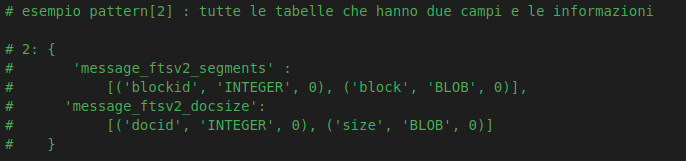
\includegraphics[scale=0.5]{assets/recovery_dict}
\end{figure}

Il dizionario ci consentirà di trovare un insieme di tabelle candidate a seconda della struttura del record trovato.

Il informazioni sullo schema delle varie tabelle varranno inoltre utilizzate dalla classe report.

\newpage

Seconda modalità:

Ogni area non allocata verrà passata alla funzione analyze\string_unallocated\string_area presente all’interno del file record\string_parser.py, la funzione per ogni valore != 0 farà partire la funzione parse\string_varint\string_to\string_record (perché potrebbe essere un possibile record o frammento di record).

La funzione parse\string_varint\string_to\string_record, per aver luogo utilizzerà inoltre l’area in bytes da analizzare convertita in variabili varint (un particolare tipo di dato utilizzato da sqlite per rappresentare numeri interi).

\medskip

Ogni record in SQLite è composto da una variabile varint rappresentante il numero di bytes del payload, una seconda variabile varint rappresentante il row id e da un insieme di byte rappresentante il payload.

Il payload si suddivide in un header e un body, l’header inizia con una variabile varint rappresentante il numero di bytes nell’header, seguita da una o più varint (una per colonna) rappresentanti i serial type che ci indicano il tipo di dato in quella colonna e la size in byte del dato.

\medskip

Terminato l’header inizia il body, tramite i serial type ottenuti precedentemente sapremo riconoscere le colonne nel body e quanti byte sono utilizzati per contenere il valore della relativa colonna.

\medskip

Ottenuto un possibile record proveremo a vedere se ci sono tabelle candidate, ovvero seguenti la medesima struttura. Se la struttura è associata ad almeno ad una tabella, aggiungo il record ottenuto al dizionario della classe report, che ci consentirà successivamente di visualizzarlo tramite una comoda interfaccia. 

\section{Interfaccia}
Dopo aver eseguito lo script, verranno prodotti tre file; un primo file contente i byte presi dalle aree in cui potrebbero essere presenti dei record rimossi, un secondo file json contenente le informazioni sull'esecuzione dello script, su i record trovati e sulle relative tabelle candidate e, infine, un terzo file html che consente la visualizzazione del file json.
Questa interfaccia è stata realizzata mediante l'utilizzo del framework boostrap. Per consentire il caricamento in modo asincrono del file json è stata usata la libreria javascript jQuery. \cite{jquery} Per rendere la pagina interattiva, sono stati gestiti una serie di eventi da parte dell'utente mediante semplici funzioni javascript.
L'interfaccia è stata resa responsive tramite la tecnologia grid-system \cite{boostrapgridsystem} fornita dal framework boostrap, in modo da essere utilizzata sia su dispositivi desktop che mobili.

\begin{figure}[ht]
	\centerline{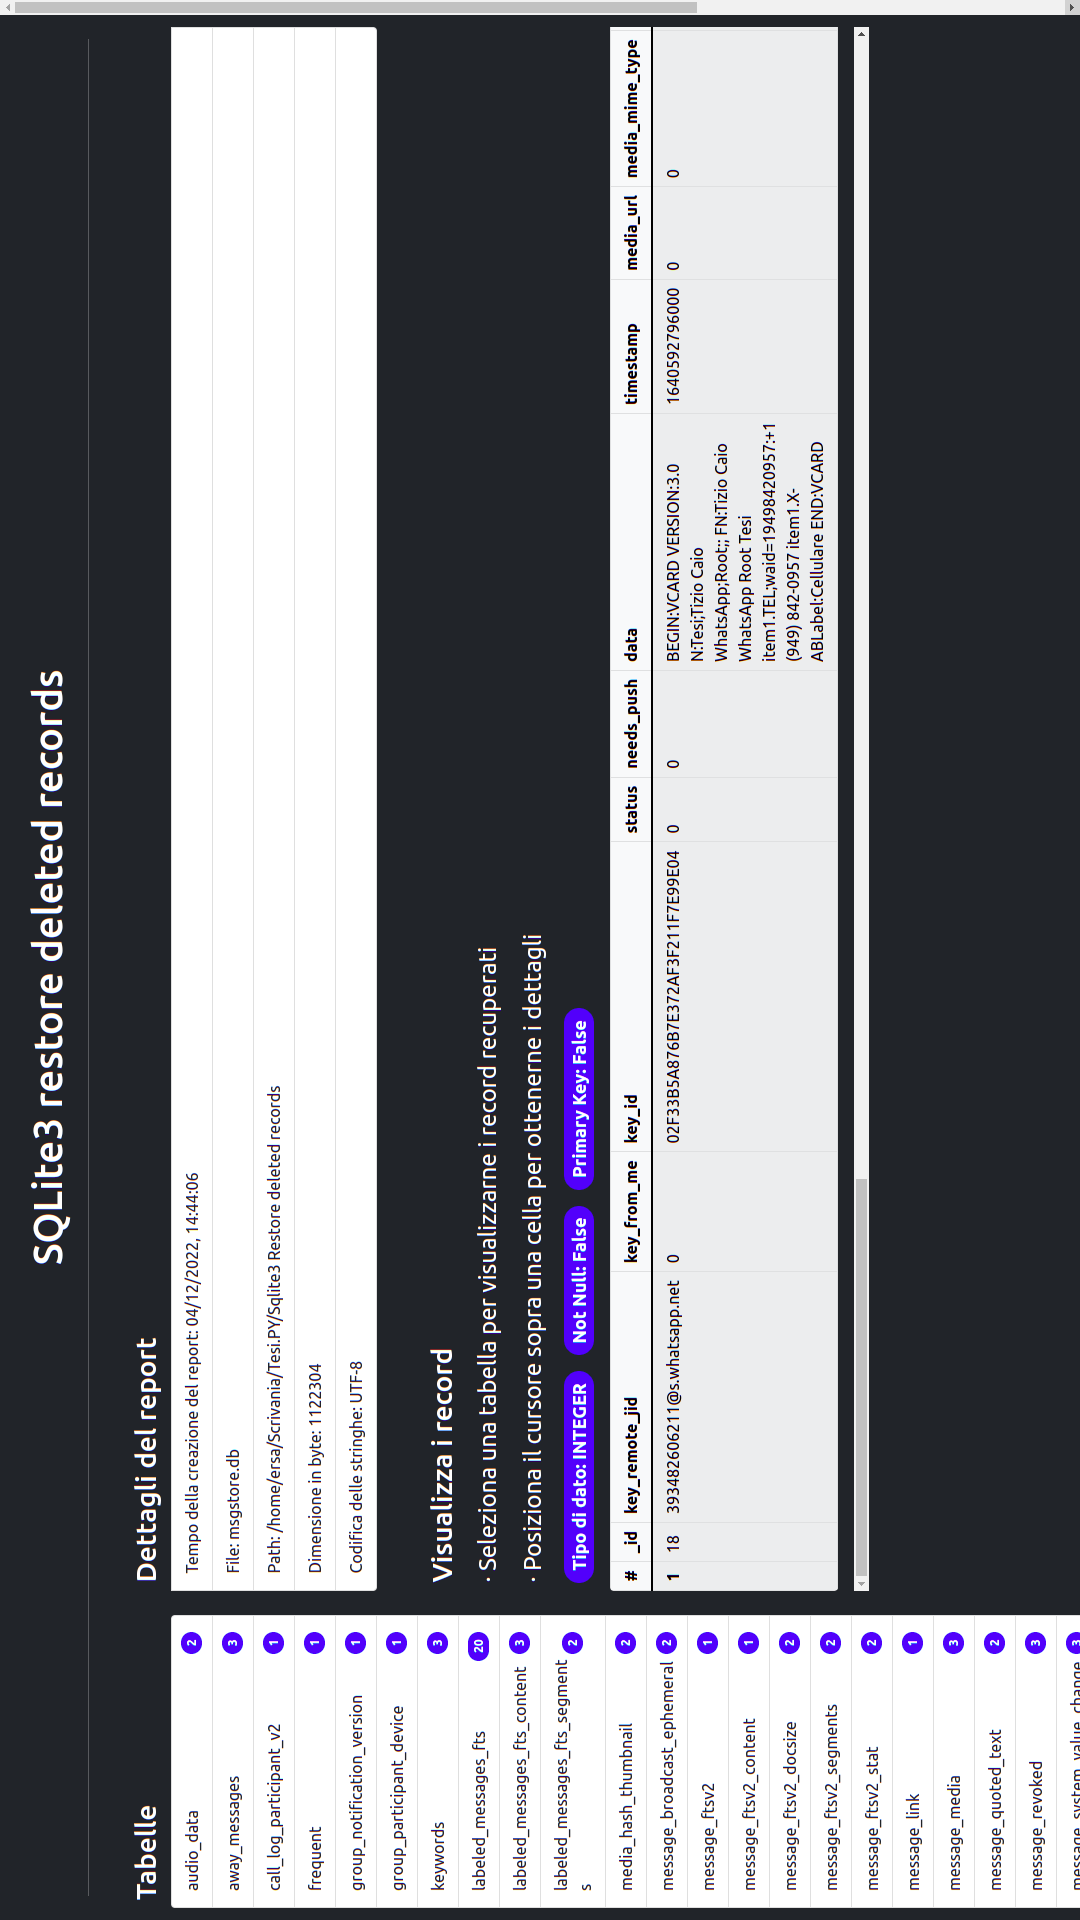
\includegraphics[scale=0.35, ]{assets/interface}}
	\caption{Interfaccia di SQLite Recovery}
	\label{fig:interface}
\end{figure}


